\begin{artengenv2auth}{Rados\l aw A. Kycia, Agnieszka Niemczynowicz}
	{Information and physics}
	{Information and physics}
	{Information and physics}
	{}
	{This is an overview article that contains the discussion of the connection between information and physics at the elementary level. We present a derivation of Landauer's bound for heat emission during irreversible logical operation. In this computation the Szilard's version of Maxwell's demon paradox is used as a model to design thermodynamic implementation of a single bit of computer memory. Landauer's principle also motivates the discussion on the practical and emergent nature of the information. Apart from physics, the principle has implications in philosophy. }
	{Landauer's principle, entropy, the second law of thermodynamics, memory, information}
	{%
		{\flushright\subbold{Rados\l aw A. Kycia}\\\subsubsectit\small{Department of Mathematics and Statistics, Masaryk Univeristy\\
		Faculty of Materials Science and Physics, Cracow University of Technology}\par}%
		{\flushright\subbold{Agnieszka Niemczynowcz}\\\subsubsectit\small{Faculty of Mathematics and Computer Science,\\
		University of Warmia and Mazury}\par}%
	}




%%%%%%%%%%%%%%%
\section{Introduction}
%%%%%%%%%%%%%%%
\lettrine[loversize=0.13,lines=2,lraise=-0.03,nindent=0em,findent=0.2pt]%
{O}{}ur civilization is based on information and creates it at a rapid rate. The common understanding of 'information' is related to:
\begin{itemize}
 \item {Representation using binary notation (for instance), i.e. two values/bits defined as $0$ and $1$, associated with 'true' and 'false', which have their own logical operations. In this approach, information represents a sequence of answers for binary questions \parencite{InformationEntropy}. This approach is adopted in current computer systems.}
 \item {Boolean algebras \parencite{InformationEntropy}. These are mathematical descriptions of logic (and information) mentioned in the previous point.}
 \item {Statistical description of information in the context of its effective encoding by the use of Shannon's information (or coding) theory \parencite{InformationEntropy}. This approach is connected with statistics and a long sequence of bits.}
\end{itemize}

The first question is therefore about the term 'information'. In general, the sequence of bits (e.g. $0101100101$) is useless unless the context in which it is produced is provided. In other words, a sequence of bits is a sequence of 'true/false' answers to specific questions. If they are 'not-overlapping', then they increase our knowledge of the nature of the subject being examined. For instance, for a question about a particular object, we can prepare the following sequence: Is it round?, Is it green?, and so forth. Each question that is substantially different from the previous yields an answer that provides us with additional knowledge about the object. This is how we gather 'information' about the world. The representation is a way how we encode this knowledge. 

Summarizing, we say that information is knowledge (sequence of answers for substantially different questions) about some objects or phenomena. It is represented by (encoded in) a sequence of letters from some alphabet. Then it can be analyzed and processed in terms of, e.g., statistical analysis or Boolean algebra. Often in literature both of these notions are merged \parencite{InformationEntropy} or the term information is related to its representation and processing without its semantic. Both these concepts are abstract, in the sense that they are not related to any physical phenomenon.

Modern computer systems exclusively use a binary representation of information. However, if one considers arbitrary base $b>1$ for representation of numbers, then according to Shannon's theory \parencite{InformationEntropy}, the information per digit is described by $\frac{ln{b}}{b}$. This function has its maximum at $b=e=2.7\ldots$, that is, the base of natural logarithms (Napier's or Euler's number). This is an irrational number and its use as a base is difficult to achieve, although not impossible \parencite{ThirdBase}. This fact has also motivated the design of computer systems based on trit ($b=3$), which is closer to optimal coding base $e$ than to the binary base ($b=2$). Due to their more complicated construction, such systems are not common. However, this example shows that the encoding we use to collect information is the second-close to optimal.

The next question concerns the nature of the information. Is it an abstract entity, or does some physical quantity represent it? Rolf Landauer \parencite*{ Landauer} first highlighted the connection between the abstract world of information presented above and its physics representation. It was later popularized by Charles H.  \textcite{Bennet}, who also proposed the application of  Landauer's principle to resolve the long-lasting paradox of Maxwell's demon \parencite{BennetDemon}. 

The principle states that during irreversible (i.e. non-bijective) computational processes,  heat is emitted in the memory. The bound for the emitted heat is given by Landauer's bound:
\begin{equation}
 Q_{L}=k_{B}T\ln{2},
 \label{Eq.LandauersBound}
\end{equation}
per bit, where $T$ is the temperature at which system operates and $k_{B}=1.380649\times 10^{-23} \frac{J}{K}$ is the Boltzmann constant. Due to the small value of $k_{B}$, this heat does not generate overheating in modern computing systems. This principle states that operations on a physical representation of information produce physical/measurable consequences.

Landauer's principle has recently undergone heavy testing \parencite{LandauerMeasurment}, including recent tests in quantum systems \parencite{QuantumLandauer}. It has also been theoretically investigated \parencites{LandauerExplained, LandauerExplainedFull, Piechocinska, ThermodynamicCostOfDataProcessing, KyciaLandauer, KyciaLandauer2} from different viewpoints. Moreover, an application to multivalued logic has been proposed \parencites{TritLandauer, KyciaNiemczynowicz}. This raises questions about the physicality of information: at which level is Landauer's heat expelled and how it is associated with the notion of information?

In this paper we present the ideas behind Landauer's principle and its connection with Maxwell's demon paradox on the elementary level. We also use some of our recent results from \parencite{KyciaNiemczynowicz} that contain a general method of constructing a higher base thermodynamic analog of memory and its connection with category theory, namely, the Galois connection. Therefore, the paper is a review and not original research. We will treat the subject elementarily, to explain Landauer's principle to the broad community of philosophers, physicists, and a general audience. We will also trace different concepts related to information: an abstract entity including its representation in terms of a sequence of letters of the alphabet, e.g., bits, and its representation in the configuration of a physical system.

The paper is organized as follows. In the next section we describe a simple version of Maxwell's demon paradox attributed to  \textcite{Szilard} and its resolution by the Landauer's principle. We then use this model to construct a single bit of thermodynamic version of computer memory. This model explains a subtle connection between information and its physical realization. This will be simplified here, with a more pedagogical version of the results presented in \parencite{KyciaNiemczynowicz}. Finally, we comment on the relationship between abstract information and its representation using physical systems. 


%%%%%%%%%%%
\section{Maxwell's demon}
%%%%%%%%%%
Maxwell's demon is a common paradox of thermodynamics that was solved only recently utilizing Landauer's principle \parencites{Landauer, Bennet, Feynman} which is currently accepted and verified experimentally solution as explained in the Introduction. The physics and philosophy literature on this subject is currently vast, and the good starting point that merges both disciplines is  \parencite{LandauerExplained}.

In this section we present a simple version of Szilard's experiment \parencites{Szilard, Feynman}, which uses a single particle of the ideal gas, with the following equation of state (for the particle) \parencites{KyciaLandauer2, LychaginThermodynamics, EivindThermodynamics}
\begin{equation}
pV=k_{B}T, 
\end{equation}
where $p$ is the pressure and $V$ is the available volume for the particle. In the experiment, all elements are 'idealized' in the sense that there are no energy losses for friction. 

Imagine that the particle of the ideal gas is inside the box of temperature $T$. The particle is in thermal equilibrium with the walls of the box. We construct a thermodynamic cycle that extracts useful work from the system. Maxwell's demon is a new system that ensures the proper course of the cycle.

In the first step of the cycle, insert a wall inside the box, dividing it into two chambers of equal volume $\frac{V}{2}$. At this stage, the demon that guides the machine cycle does not know in which part of the box the particle can be found. The situation is presented in Fig. \ref{Fig.Szilard_StateUnknown}.
%%%%%%%%%%%
\begin{figure}
\centering
 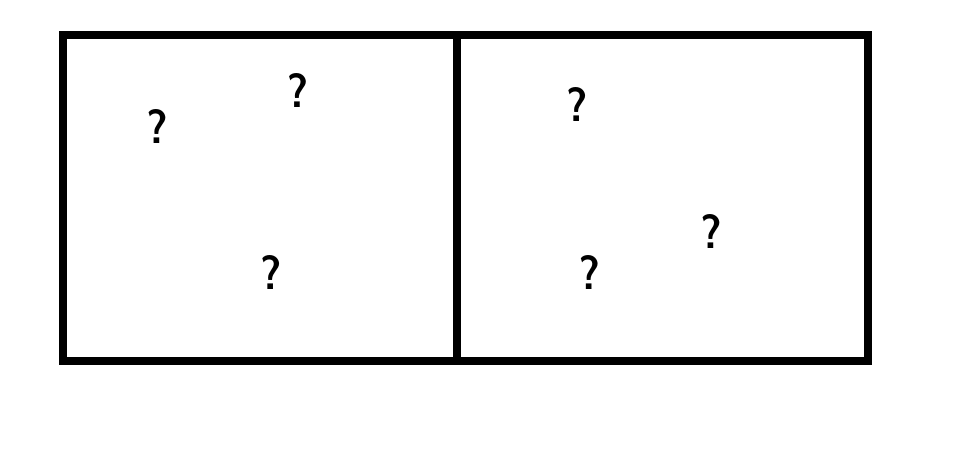
\includegraphics[width=0.5\textwidth]{ART_Kycia_Niemczynowicz/Demon1.png}
 \caption{The box split in half, with the unknown location of a particle.}
 \label{Fig.Szilard_StateUnknown}
\end{figure}
%%%%%%%%%%%

To start extracting useful work, the demon must locate the particle, or in other words, gain and store information about particle location. The situation after localizing the particle is presented in Fig. \ref{Fig.Szilard_ParticleLocated}.
%%%%%%%%%%%
\begin{figure}
\centering
 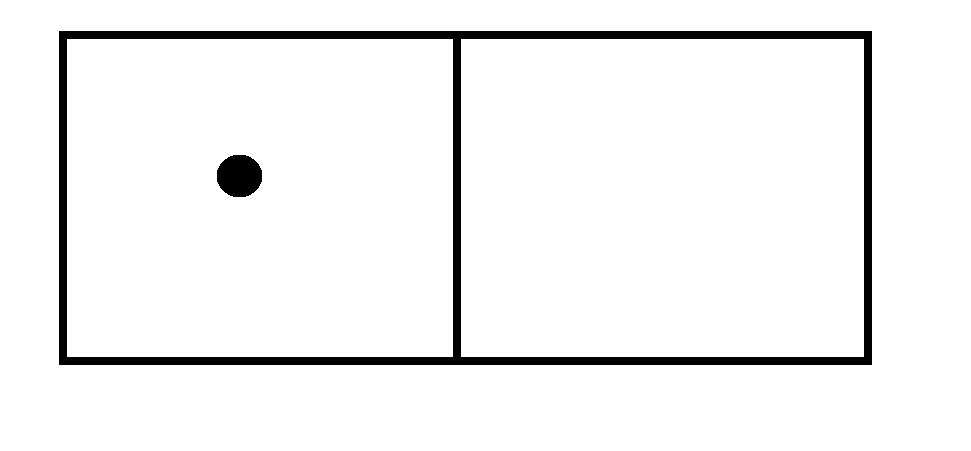
\includegraphics[width=0.5\textwidth]{ART_Kycia_Niemczynowicz/Demon2.png}
 \caption{In this case the particle is located in the left chamber of the box.}
 \label{Fig.Szilard_ParticleLocated}
\end{figure}
%%%%%%%%%%%

In the next step, the border between the chambers become movable. Energy is extracted when the gas is decompressed isothermally. This decompression is a reversible thermodynamic process and the work done by the particle is given by: 
\begin{equation}
 W=k_{B}T\int_{V/2}^{V}=k_{B}T \ln{2}.
\end{equation}
The situation is presented in Fig. \ref{Fig.Szilard_WorkExtraction}.
%%%%%%%%%%%
\begin{figure}
\centering
 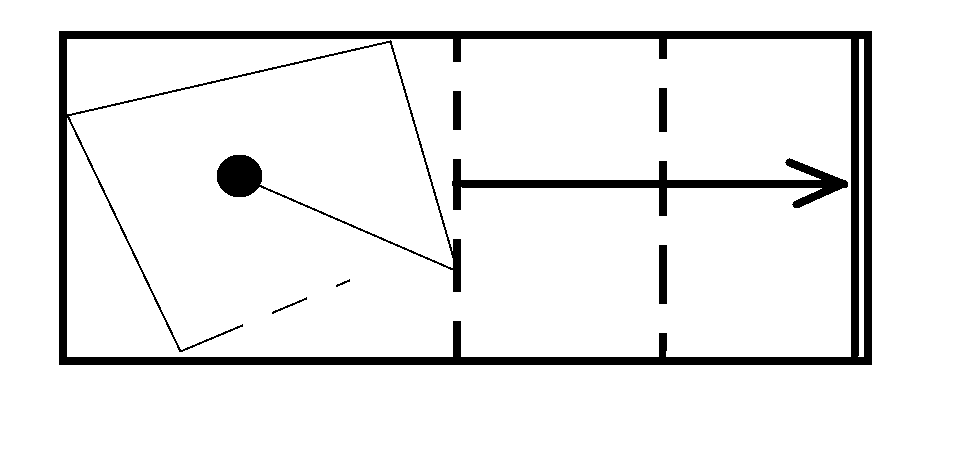
\includegraphics[width=0.5\textwidth]{ART_Kycia_Niemczynowicz/Demon3.png}
 \caption{Energy extraction in the isothermal expansion of a single particle of the ideal gas.}
 \label{Fig.Szilard_WorkExtraction}
\end{figure}
%%%%%%%%%%%

The final part of the cycle is the restart. The demon takes the border out of the box, moves it and then re-insert it again in the middle. We return here to the situation from Fig. \ref{Fig.Szilard_StateUnknown}. At this stage, information about the particle location is not needed, so the demon must delete it to return the whole system (box and demon) to the initial state for another round of the cycle. Therefore, we now have the same state as at the beginning of the previous turn.

This situation can be analyzed in terms of the second law of thermodynamics and entropy $S$. The second law of thermodynamics says that the change of total entropy (system and environment) must be non-decreasing.

In the case above, in the cycle, according to the conservation of energy (the first law of thermodynamics), the heat from the environment (the thermal bath of the particle) is extracted and used to make work $W$. Therefore, the deficiency of heat is $Q=W=k_{B}T\ln(2)$. Given that the balance is negative and the system is held at a constant temperature, the entropy change in the cycle is
\begin{equation}
 \Delta S = -\frac{Q}{T}=-k_{B}\ln(2) <0.
\end{equation}
This contradicts the second law (it must be $\Delta S \geq0$).

To solve this apparent contradiction,  \textcites{BennetDemon} has suggested that during the demon's erasure of the bit of information regarding particle location (say $0$--the particle in the left chamber, $1$--the particle in the right chamber) the heat of value $Q_{e}$ is expelled. This heat is no less than Landauer's bound (\ref{Eq.LandauersBound}), that is $Q_{e} \geq Q_{L}$. This assumption corrects the balance of entropy:
\begin{equation}
 \Delta S = \frac{Q_{e}}{T}-\frac{Q}{T} \geq k_{B}\ln(2) - k_{B}\ln(2) =0.
\end{equation}

Bennett's explanation solves the long-standing paradox by employing Landauer's idea. It is interesting to note that the paradox remained unresolved until the 1970s. Moreover, its resolution is based on the idea of information, computing, and memory developed in the twentieth century and therefore not known to the fathers of thermodynamics. The solution can almost be regarded as manifest in the works of \textcites{Szilard} if his experiment is interpreted as a model for computer memory. This reinterpretation of Szilard's results is presented in the next section, which provides a more in-depth insight into the connection between information and its implementation.

%%%%%%%%%%%%%%%%%%%%%%%
\section{Memory}
%%%%%%%%%%%%%%%%%%%%%%%
Szilard's \textit{gedanken experiment} presented in the previous section can be used to construct a thermodynamic model of computer memory. We consider here the simplest case; a more detailed presentation for general memory for multivalued logic is given in \parencite{KyciaNiemczynowicz}.

The implementation of a single bit thermodynamic memory is presented in Fig. \ref{Fig.BinaryCell}.
%%%%%%%%%%%
\begin{figure}
\centering
 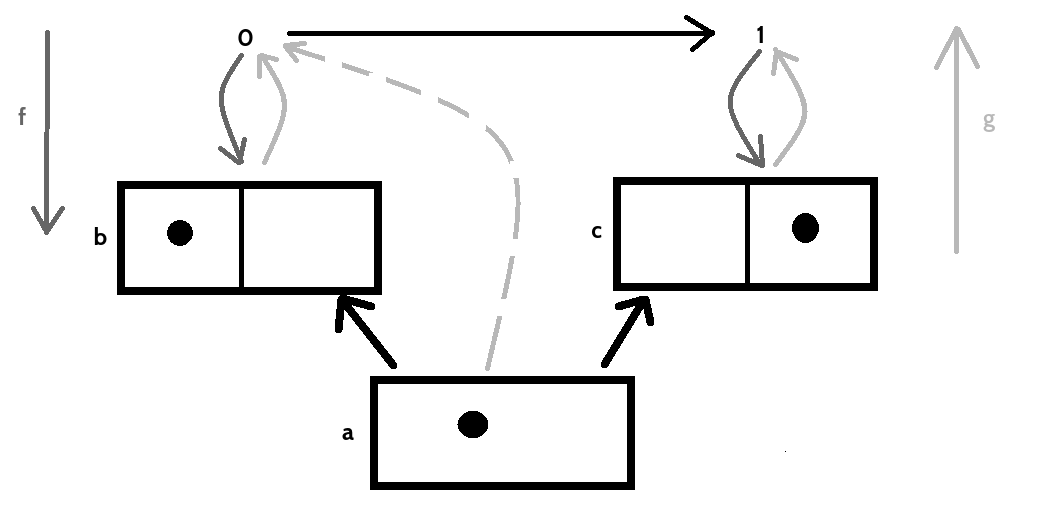
\includegraphics[width=0.7\textwidth]{ART_Kycia_Niemczynowicz/BinaryGalois-bw.png}
 \caption{Implementation of memory using the thermodynamic model of the reversed Szilard's model of Maxwell's demon. State $a$ is not associated with logical value: it is an undetermined internal state of the memory, which can be associated with $0$ at the logical level. State $b$ represents $0$, and state $c$ represents $1$. Maps $f$ and $g$, associating logical values with their physical implementation, are selected in such a way to preserve the order indicated by black lines representing transitions between states or ordering in Boolean algebra, that is, logic. This is a reminiscence of the Galois connection \parencite{SpivakSketches, CategoryGentleIntroduction, KyciaLandauer} that usually occurs where there is a system that contains an abstract level and its implementation.}
 \label{Fig.BinaryCell}
\end{figure}
%%%%%%%%%%%

State $a$ is an inner state of memory that does not represent any logical value. It is used to implement all logical operations (not necessarily those that swap $0$ and $1$). This assumption is consistent with the previous discussion of Szilard's model and its reverse. 

We can now proceed to a detailed description of the types of operations. At the level of logic, we have two types of operations on this memory:
\begin{itemize}
 \item {Reversible: operations that have inverses, i.e., those that are bijections, for instance, a NOT gate whose function is involutive: $0  \leftrightarrow 1$.}
 \item {Irreversible: operations that do not have inverse, for instance the assignment of some value that 'forgets' the previous value: ($0 \rightarrow 1$, $1 \rightarrow 1)$.}
\end{itemize}

At the level of thermodynamics, we have a similar convention. However, the definition is different:
\begin{itemize}
 \item {Reversible: realized by reversible thermodynamic processes, i.e. processes that can be reversed, or equivalently, the process that combined into a cycle with its inverse has vanishing entropy change $\Delta S =0$.}
 \item {Irreversible: realized by irreversible thermodynamic processes, i.e. if we perform this operation and then return (along any reversible process) to the initial state, then in the cycle $\Delta S >0$.}
\end{itemize}


As highlighted in \parencite{LandauerExplained}, the main idea behind Landauer's principle is the association of operations at the level of logic and their physical implementation in the form presented in Tab. \ref{Tab.LandauerConnection}; in our case, $A$ is the logical system and $B$ is its memory implementation.
%%%
\begin{table}
\centering
\begin{tabular}[!h]{|c|c|c|}
 \hline
 Possibilities &  \begin{tabular}{@{}c@{}}$B$ \\ reversible\end{tabular}  & \begin{tabular}{@{}c@{}}$B$ \\ irreversible\end{tabular} \\ \hline
 $A$ reversible & YES  & YES \\ \hline
 $A$ irreversible & NO & YES \\ \hline
\end{tabular}
\caption{Systems $A$ is implemented on $B$.} 
\label{Tab.LandauerConnection}
\end{table}
%%%


To understand this association, we provide some examples of logical operations and their physical implementations. 

To assign some initial value to memory state, let us start from state $a$ and perform isothermal compression to $b$. This initial preparation expels (stores) the heat $Q=k_{B}T\ln(2)$ to(in) the environment and sets the initial logical state to $0$.

Consider the reversible NOT operation. According to Tab. \ref{Tab.LandauerConnection}, this can be realized in two inequivalent thermodynamically ways at the physical level:
\begin{enumerate}
 \item {Reversible thermodynamic operation: isothermal expansion $b \rightarrow a$ and then isothermal compression $a \rightarrow c$. The composed operation is thermodynamically reversible and no heat is expelled to the environment or converted to work.}
 \item {Irreversible thermodynamic operation: we take the middle border out of the box, which generates free adiabatic decompression of the gas (particle) $b \rightarrow a$. Next, reversible isothermal compression $a \rightarrow c$ is made. When the first step is performed, we lose 'access' to the heat initially stored in $0$ state. This heat cannot be regained/reused and therefore must be treated as Landauer's heat.}
\end{enumerate}


Consider now the irreversible logical operation of setting $1$ starting from $0$. According to Tab. \ref{Tab.LandauerConnection}, this must be realized by an irreversible thermodynamic operation and hence it is the same as the operation from the second point above. Therefore, Landauer's heat is also expelled in this case.

This example is also proof that Landauer's principle is equivalent (at least for these examples) to the association from Tab. \ref{Tab.LandauerConnection} between operations on logical and thermodynamic states.


The presentation in this section was elementary, intending to be an introduction to the multivalued logic approach \parencites{KyciaNiemczynowicz, TritLandauer}, category theory formulation of this principle \parencites{KyciaLandauer, KyciaLandauer2}, mentioned briefly above, and its understanding in more fundamental level \parencite{LandauerExplained}. We also emphasize that the principle can be thoroughly understood only at the level of statistical physics \parencites{LandauerExplainedFull, Piechocinska}, and equilibrium thermodynamics used above is only its limiting case.

In the following conclusion section we briefly discuss the nature of information.


%%%%%%%%%%%%%%%
\section{Discussion}
%%%%%%%%%%%%%%%

The thermodynamic realization of a bit of information is a simple model that presents how Landauer's heat is generated for irreversible operations. In this model, energy is initially stored in the environment by setting some starting value ($0$ or $1$) in the memory. An irreversible operation then makes it impossible to reuse/regain this heat to perform work and thus extract energy from the memory to gain the initially 'invested' energy. In this interpretation, a bit labels the state of a system that contains energy that can be accessed and (re)used. Reversible operations are designed to extract this energy, whereas irreversible ones lose it. Therefore, according to the laws of thermodynamics, for irreversible operation, heat is expelled. 

Abstracting even more, the information is stored in some sort of energy configuration of the physical system. From the mathematical viewpoint, there is an abstract notion of information (bits, Boolean algebras), but ultimately information must be represented by certain physical states, allowing it to interact with the physical world. This storing process of information forms a connection between its abstract notion and the physical world.

This also has some practical consequences to philosophy. The 'sacrum' (abstraction) cannot be separated from 'profane' (realization). Abstract concepts (encoded as some form of information) must always be stored in some physical configuration of matter/energy. Information is a type of emergent concept or a new complexity built on top of physical constructs and our ability to manipulate energy and matter. This is a highly pragmatic approach. 

This perspective shows that information, although immaterial concept, exists in the Universe as its encoding/representation in physical content of matter and energy. Their properties can be abstracted, however, we always deal and interact with some of its representation. The connection between abstract notion and its multiple (physical) representations is also reflected in the Galois connection \parencite{CategoryGentleIntroduction}---a process of abstraction---which can be seen as a modern allegory of Plato's cave---a projection of mathematical (ideal) entity to the concrete realization (shadow on the cave wall).



%%%%%%%%%%%%%%%
\section{Conclusion}
%%%%%%%%%%%%%%%
We presented an overview of the basic facts from the thermodynamics of Maxwell's demon, its model by Szilard and the resolution of this paradox by Landauer. This motivated us to consider the correspondence between information and its physical representation. The aim was to introduce a broad audience to the basics of this subject and provide some references that can be used for more in-depth studies.


%%%%%%%%%%%%%%%%%%%%%%%%

\paragraph{Acknowledgments} We would like to thank anonymous Referees for useful comments and remarks that helped us improve the paper.

RK was supported by the GACR grant GA19-06357S, the grant 8J20DE004 of Ministry of Education, Youth and Sports of the CR, and Masaryk University grant MUNI/A/0885/2019. We would like to acknowledge COST CA18223 action for support.

 
 \end{artengenv2auth}

